\documentclass{article}
\usepackage[utf8]{inputenc}
\usepackage{amsmath}
\usepackage[margin=1cm]{geometry}
\usepackage[english]{babel} % English language/hyphenation
\usepackage{amsmath,amsthm,amssymb}
\usepackage{setspace}
\usepackage{breqn}
\usepackage{enumerate}
\usepackage{multicol}
\usepackage{pgfplots}


\theoremstyle{definition}
\newtheorem{theorem}{Exercise}[section]

\theoremstyle{remark}
\newtheorem*{claim}{Claim}

\newcommand{\R}{\mathbb{R}}
\newcommand{\Z}{\mathbb{Z}}
\newcommand{\N}{\mathbb{N}}
\newcommand{\inv}[1]{#1^{-1}}
\setcounter{section}{3}

\doublespacing
\begin{document}
	\begin{flushright}
		Moshe Mason Rubin\\MATH 330 Homework \#5\\3 October 2016
	\end{flushright}

	\setcounter{section}{4}
	\setcounter{theorem}{13}
	\begin{theorem}
		Let \[A=\begin{bmatrix}
		0 & 1 \\ 
		-1 & 0
		\end{bmatrix} \text{ and } B=\begin{bmatrix}
		0 & -1 \\ 
		1 & -1
		\end{bmatrix} \] be elements in $GL_2\left(\R\right)$.Show that $A$ and $B$ have finite orders but $AB$ does not. 
	\end{theorem}
	\begin{proof}
		Notice 
		\begin{dgroup*}
			\begin{dmath*}
				A^2 \hiderel{=} \begin{bmatrix}
					0 & 1 \\ 
					-1 & 0
				\end{bmatrix}\begin{bmatrix}
					0 & 1 \\ 
					-1 & 0
				\end{bmatrix} \hiderel{=} \begin{bmatrix}
					-1 & 0 \\ 
					0 & -1
				\end{bmatrix} 
			\end{dmath*}
			\begin{dsuspend}
				and
			\end{dsuspend}
			\begin{dmath*}
				A^4 \hiderel{=} A^2A^2 = \begin{bmatrix}
					-1 & 0 \\ 
					0 & -1
				\end{bmatrix} \begin{bmatrix}
					-1 & 0 \\ 
					0 & -1
				\end{bmatrix} = \begin{bmatrix}
					1 & 0 \\ 
					0 & 1
				\end{bmatrix} \hiderel{=} id
			\end{dmath*}
			\begin{dsuspend}
				so $A$ is of order $4$. Notice 
			\end{dsuspend}
			\begin{dmath*}
				B^3 = \begin{bmatrix}
					0 & -1 \\ 
					1 & -1
				\end{bmatrix}\begin{bmatrix}
					0 & -1 \\ 
					1 & -1
				\end{bmatrix}\begin{bmatrix}
					0 & -1 \\ 
					1 & -1
				\end{bmatrix} = \begin{bmatrix}
					-1 & 1 \\ 
					-1 & 0
				\end{bmatrix} \begin{bmatrix}
					0 & -1 \\ 
					1 & -1
				\end{bmatrix} = \begin{bmatrix}
					1 & 0 \\ 
					0 & 1
				\end{bmatrix} \hiderel{=} id
			\end{dmath*}
		\end{dgroup*} So $B$ is of order $3$. \\
		Notice $AB=\left[\begin{smallmatrix}
			1 & -1 \\ 
			0 & 1
		\end{smallmatrix} \right]$
		\begin{claim}
			$\left(AB\right)^n=\left[\begin{smallmatrix}
			1 & -n \\ 
			0 & 1
			\end{smallmatrix} \right]$ for $n\in\N$, so $AB$ is of infinite order as this would imply there is no $n\in\N$ such that $\left(AB\right)^n=id$. 
			
			By induction:
			\begin{description}
				\item[Base case] $n=2$:\\
				\begin{dmath*}
					\left(AB\right)^2 = \begin{bmatrix}
						1 & -1 \\ 
						0 & 1
					\end{bmatrix}\begin{bmatrix}
						1 & -1 \\ 
						0 & 1
					\end{bmatrix} = \begin{bmatrix}
						1 & -2 \\ 
						0 & 1
					\end{bmatrix} 
				\end{dmath*} So the hypothesis holds for $n=2$. \checkmark
			
				\item[Inductive step] Assume $\left(AB\right)^n=\left[\begin{smallmatrix}
					1 & -n \\ 
					0 & 1
				\end{smallmatrix} \right]$ for some fixed $n\in\N$ and show that $\left(AB\right)^{n+1}=\left[\begin{smallmatrix}
					1 & -\left(n+1\right) \\ 
					0 & 1
				\end{smallmatrix} \right]$:\\
				\begin{dmath*}
					\left(AB\right)^{n+1} = \left(AB\right)^n\left(AB\right) = \begin{bmatrix}
						1 & -n \\ 
						0 & 1
					\end{bmatrix} \begin{bmatrix}
						0 & -1 \\ 
						0 & 1
					\end{bmatrix} = \begin{bmatrix}
						1 & -1-n \\ 
						0 & 1
					\end{bmatrix} \hiderel{=} \begin{bmatrix}
						1 & -\left(n+1\right) \\ 
						0 & 1
					\end{bmatrix} \condition[]{\checkmark} 
				\end{dmath*}
			\end{description} So $\left(AB\right)^n=\left[\begin{smallmatrix}
				1 & -n \\ 
				0 & 1
			\end{smallmatrix} \right]$ for $n\in\N$.
		\end{claim}
		So $AB$ is of infinite order as this would imply there is no $n\in\N$ such that $\left(AB\right)^n=id$. 
	\end{proof}
	
	\setcounter{theorem}{17}
	\begin{theorem} Calculate each of the following expressions.
		\begin{multicols}{4} 
			\noindent
			\begin{enumerate}[(a)]
				\item $\inv{\left(1+i\right)}$
				\item $\left(1+i\right)^6$
				\item $\left(\sqrt{3}+i\right)^5$
				\item $\left(-i\right)^{10}$
				\item $\left(\frac{1-i}{2}\right)^4$
				\item $\left(-\sqrt{2}-\sqrt{2}i\right)^{12}$
				\item $\left(-2+2i\right)^{-5}$
			\end{enumerate}
		\end{multicols} 
	\end{theorem}
	\begin{proof} Recall that \textit{Euler's Formula} that  $Ae^{i\theta}=A\left(\cos\theta+i\sin\theta\right)$ for $A\in\R$, $\theta\in\left[0,2\pi\right]$.
		\begin{enumerate}[(a)]
			\item $\inv{\left(1+i\right)}$ is given by $\frac{1}{2}-\frac{1}{2}i$ as $\left(1+i\right)\left(\frac{1}{2}-\frac{1}{2}i\right)=\frac{1}{2}-\frac{1}{2}i+\frac{1}{2}i+\frac{1}{2}=1$. So \fbox{$\frac{1}{2}-\frac{1}{2}i=\inv{\left(1+i\right)}$}.
			
			\item By \textit{Euler's Formula}, $1+i=\sqrt{2}e^{\frac{i\pi}{4}}$, so 
			\begin{dmath*}
				\left(1+i\right)^6 = \left(\sqrt{2}e^{\frac{i\pi}{4}}\right)^6 = \sqrt{2}^6e^{\frac{6i\pi}{4}} = 8 e^{\frac{3i\pi}{2}} = 8\left(\cos\left(\frac{3\pi}{2}\right)+i\sin\left(\frac{3\pi}{2}\right)\right) \condition[]{by \textit{Euler's Formula}}= -8i \condition{as $\cos\left(\frac{3\pi}{2}\right)=0$ and $\sin\left(\frac{3\pi}{2}\right)=-1$}
			\end{dmath*}
			So \fbox{$\left(1+i\right)^6=-8i$}. 
			
			\item By \textit{Euler's Formula}, $\sqrt{3}+i=2e^{\frac{i\pi}{6}}$, so
			\begin{dmath*}
				\left(\sqrt{3}+i\right)^5 = \left(2e^{\frac{i\pi}{6}}\right)^5 = 2^5 e^{\frac{5i\pi}{6}} = 32\left(\cos\left(\frac{5\pi}{6}\right)+i\sin\left(\frac{5\pi}{6}\right)\right) \condition[]{by \textit{Euler's Formula}}= 32\left(-\frac{\sqrt{3}}{2}+\frac{1}{2}i\right) \condition[]{ as $\cos\left(\frac{5\pi}{6}\right)=-\frac{\sqrt{3}}{2}$ and $\sin\left(\frac{5\pi}{6}\right)=\frac{1}{2}$} = 16i-16\sqrt{3}
			\end{dmath*} So \fbox{$\left(\sqrt{3}+i\right)^5 = 16i-16\sqrt{3}$}. 
			
			
			\item \begin{dmath*}
				\left(-i\right)^{10} = \left(-1\right)^{10}\left(i\right)^{10} = \left(-1\right)^2\left(i\right)^2 \condition[]{as $\left(-1\right)^m=\left(-1\right)^{\left(m\bmod 2\right)}$ and $i^n=i^{\left(n\bmod 4\right)}$} = \left(1\right)\left(-1\right) = -1
			\end{dmath*} So \fbox{$\left(-i\right)^{10}=-1$}. 
		
			\item By \textit{Euler's Formula}, $\frac{1-i}{2} = \frac{1}{2}-\frac{1}{2}i = \frac{\sqrt{2}}{2}e^{\frac{7i\pi}{4}}$, so 
			\begin{dmath*}
				\left(\frac{1-i}{2}\right)^4 = \left(\frac{\sqrt{2}}{2}e^{\frac{7i\pi}{4}}\right)^4 = \left(\frac{\sqrt{2}}{2}\right)^4 e^{7i\pi} = \frac{1}{4}e^{i\pi} \condition[]{as we restrict $\theta$ to $0\leq\theta\leq2\pi$} = \frac{1}{4}\left(\cos\left(\pi\right)+i\sin\left(\pi\right)\right) = -\frac{1}{4}
			\end{dmath*} So \fbox{$\left(\frac{1-i}{2}\right)^4=-\frac{1}{4}$}. 
		
			
			\item By \textit{Euler's Formula}, $-\sqrt{2}-\sqrt{2}i=2e^{\frac{5i\pi}{4}}$, so 
			\begin{dmath*}
				\left(-\sqrt{2}-\sqrt{2}i\right)^{12} = \left(2e^{\frac{5i\pi}{4}}\right)^{12} = 2^{12} e^{\frac{60i\pi}{4}} = 4096 e^{15i\pi} = 4096e^{i\pi} \condition[]{as we restrict $\theta$ to $0\leq\theta\leq2\pi$} = -4096 \condition[]{as $e^{i\pi}=-1$ from above}
			\end{dmath*} So \fbox{$\left(-\sqrt{2}-\sqrt{2}i\right)^{12} = -4096$}. 
		
		
			\item By \textit{Euler's Formula}, $-2+2i=2\sqrt{2}e^{\frac{3i\pi}{4}}$, so
			\begin{dmath*}
				\left(-2+2i\right)^{-5} = \left(2\sqrt{2}e^{\frac{3i\pi}{4}}\right)^{-5} = \left(2\sqrt{2}\right)^{-5}\left(e^{\frac{3i\pi}{4}}\right)^{-5} = \frac{\sqrt{2}}{256}e^{\frac{-15i\pi}{4}} = \frac{\sqrt{2}}{256} e^{\frac{i\pi}{4}} \condition[]{as we restrict $\theta$ to $0\leq\theta\leq2\pi$} = \frac{\sqrt{2}}{256}\left(\frac{1}{\sqrt{2}}+\frac{1}{\sqrt{2}}i\right) \condition[]{by \textit{Euler's Formula}, as $\sin\left(\frac{\pi}{4}\right)=\cos\left(\frac{\pi}{4}\right)=\frac{1}{\sqrt{2}}$} = \frac{1}{256}+\frac{1}{256}i
			\end{dmath*} So \fbox{$\left(-2+2i\right)^{-5} = \frac{1}{256}+\frac{1}{256}i$}. \qedhere
		\end{enumerate}
	\end{proof}


	\setcounter{theorem}{19}
	\begin{theorem}
		List and graph that $6^{\textit{th}}$ roots of unity. What are the generators of this group? What are the primitive $6^{\textit{th}}$ roots of unity? 
	\end{theorem}
	\begin{proof} By Theorem 4.11, the $6^{\textit{th}}$ roots of unity are given by $z=\cos\left(\frac{k\pi}{3}\right)+i\sin
		\left(\frac{k\pi}{3}\right)$ for $k=0,1,2,3,4,5$. So the $6^{\textit{th}}$ roots of unity are 
		\begin{multicols}{3}
			\begin{enumerate}
				\item $\cos\left(0\right)+i\sin\left(0\right)=1$
				\item $\cos\left(\frac{\pi}{3}\right)+i\sin\left(\frac{\pi}{3}\right)=\frac{1}{2}+\frac{\sqrt{3}}{2}i$
				\item $\cos\left(\frac{2\pi}{3}\right)+i\sin\left(\frac{2\pi}{3}\right)=-\frac{1}{2}+\frac{\sqrt{3}}{2}i$
				\item $\cos\left(\pi\right)+i\sin\left(\pi\right)=-1$
				\item $\cos\left(\frac{4\pi}{3}\right)+i\sin\left(\frac{4\pi}{3}\right)=-\frac{1}{2}-\frac{\sqrt{3}}{2}i$
				\item $\cos\left(\frac{5\pi}{3}\right)+i\sin\left(\frac{5\pi}{3}\right)=\frac{1}{2}-\frac{\sqrt{3}}{2}i$
			\end{enumerate}
		\end{multicols}
		Only $\frac{1}{2}+\frac{\sqrt{3}}{2}i$ and $\frac{1}{2}-\frac{\sqrt{3}}{2}i$ are primitive $6^{\textit{th}}$ roots of unity as $1^1=1$, $\left(-\frac{1}{2}+\frac{\sqrt{3}}{2}i\right)^3=1$, $\left(-1\right)^2=1$, and $\left(-\frac{1}{2}-\frac{\sqrt{3}}{2}i\right)^3=1$ for the other roots. So $\frac{1}{2}+\frac{\sqrt{3}}{2}i$ and $\frac{1}{2}-\frac{\sqrt{3}}{2}i$ are the generators of this group.\qedhere\\
		
		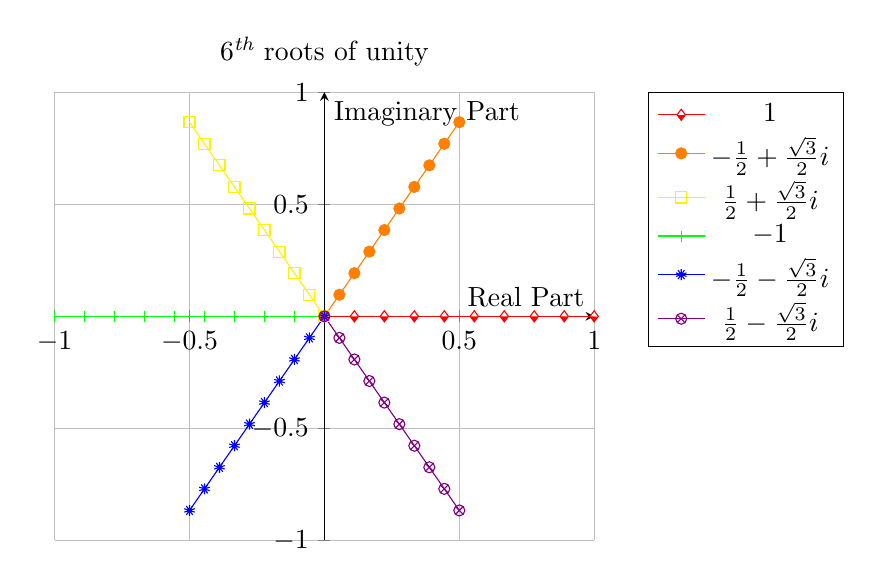
\begin{tikzpicture}
		\begin{axis}[
		title=$6^{\textit{th}}$ roots of unity,
		grid=both,
		axis lines = center,
		xlabel = Real Part,
		ylabel = {Imaginary Part},
		legend style={at={(1.1,1)},
		anchor=north west, },
		xmin=-1, xmax=1,
		ymin=-1, ymax=1,
		]
		%Below the red parabola is defined
		
		\addplot [
		domain=0:1, 
		samples=10, 
		color=red,
		mark=halfdiamond*
		]
		{0};
		\addlegendentry{$1$}
		
		\addplot [
		%		samples=10, 
		color=orange,
		mark=*
		][domain=0:0.5,samples=10]
		{1.732050808*(x-.5)+0.8660254038};
		\addlegendentry{$-\frac{1}{2}+\frac{\sqrt{3}}{2}i$}
		
		\addplot [
		domain=-.5:0, 
		samples=10, 
		color=yellow,
		mark=square
		]
		{-1.732050808*(x+.5)+0.8660254038};
		\addlegendentry{$\frac{1}{2}+\frac{\sqrt{3}}{2}i$}
		%Here the blue parabloa is defined
		

		
		\addplot [
		domain=-1:0, 
		samples=10, 
		color=green,
		mark=|
		]
		{0};
		\addlegendentry{$-1$}
		
		\addplot [
		domain=-.5:0, 
		samples=10, 
		color=blue,
		mark=10-pointed star
		]
		{1.732050808*(x+.5)-0.8660254038};
		\addlegendentry{$-\frac{1}{2}-\frac{\sqrt{3}}{2}i$}
		
		\addplot [
		domain=0:0.5, 
		samples=10, 
		color=violet,
		mark=otimes
		]
		{-1.732050808*(x-.5)-0.8660254038};
		\addlegendentry{$\frac{1}{2}-\frac{\sqrt{3}}{2}i$}
		\end{axis}
		\end{tikzpicture}	
	\end{proof}


	\setcounter{theorem}{22}
	\begin{theorem}
		Let $a,b\in G$. Prove the following statements.
		\begin{enumerate}[(a)]
			\item The order of $a$ is the same as the order of $\inv{a}$.
			\item For all $g\in G$, $|a|=|\inv{g}ag|$. 
			\item The order of $ab$ is the same as the order of $ba$. 
		\end{enumerate}
	\end{theorem}
	\begin{proof}\hfill
		\begin{enumerate}[(a)]
			\item \begin{itemize}
				\item Assume $a\in G$ is of finite order $k\in\N$. Then $a^k=1$ by definition. Then 
				\begin{dmath*}
					\left(\inv{a}\right)^k = a^{-k} \condition[]{by Theorem 3.8.2} = \inv{\left(a^k\right)} \condition[]{by Theorem 3.8.2} = \inv{\left(1\right)} \condition[]{by assumption that $a$ is of order $k$} = 1
				\end{dmath*}
				So $\left(\inv{a}\right)^k=1$. So $\inv{a}$ is of order $k$. 
				
				\item Assume $a$ is of infinite order. Then there does not exist $k\in\N$ suck that $a^k=1$. Now, assume we wish to find $n\in\N$ such that $\left(\inv{a}\right)^n=1$. Then
				\begin{dmath*}
					\left(\inv{a}\right)^n \hiderel{=} 1 \implies a^{-n} \hiderel{=} 1 \condition[]{by Theorem 3.8.2} \implies \inv{\left(a^n\right)} \hiderel{=} 1 \implies \inv{\left(a^n\right)} \hiderel{=} \left(a^n\right)\inv{\left(a^n\right)} \condition[]{by definition of $\inv{\left(a^n\right)}$} \implies 1 \hiderel{=} a^n \condition[]{by right multiplying by $a^n$}
				\end{dmath*} But $a^n\not=1$ for all $n\in\N$ by assumption that $|a|=\infty$. So $\left(\inv{a}\right)^n\not=1$ for all $n\in\N$, so $|\inv{a}|=\infty$. 
			\end{itemize}
			So $|a|=|\inv{a}|$. \qed

			\item I will show $|a|=|\inv{g}ag|$ for all $g\in G$ using the following claim:
			\begin{claim}
				$\left(\inv{g}ag\right)^k=\inv{g}a^kg$ for $k\in\N$. \\
				By induction:\nopagebreak
				\begin{description}
					\item[Base Case] $n=2$:\\
					\begin{dmath*}
						\left(\inv{g}ag\right)^2 = \left(\inv{g}ag\right)\left(\inv{g}ag\right) = \left(\inv{g}a\right)\left(g\inv{g}\right)\left(ag\right) \condition[]{by associative property} = \left(\inv{g}a\right)\left(ag\right) \condition[]{by definition of $\inv{g}$} = \inv{g}a^2g \condition[]{by associative property}
					\end{dmath*} So the hypothesis holds for $n=2$. \checkmark 
				
					\item[Inductive step] Assume $\left(\inv{g}ag\right)^k=\inv{g}a^kg$ for some fixed $k\in\N$ and show that $\left(\inv{g}ag\right)^{k+1}=\inv{g}a^{k+1}g$:
					\begin{dmath*}
						\left(\inv{g}ag\right)^{k+1} = \left(\inv{g}ag\right)^k\left(\inv{g}ag\right) = \left(\inv{g}a^kg\right)\left(\inv{g}ag\right) \condition[]{by inductive hypothesis} = \left(\inv{g}a^k\right)\left(g\inv{g}\right)\left(ag\right) \condition[]{by associative property} = \left(\inv{g}a^k\right)\left(ag\right) \condition[]{by definition of $\inv{g}$} = \inv{g}a^{k+1}g \condition[]{\checkmark}
					\end{dmath*} 
				\end{description} So $\left(\inv{g}ag\right)^k=\inv{g}a^kg\implies\left(\inv{g}ag\right)^{k+1}=\inv{g}a^{k+1}g$. So $\left(\inv{g}ag\right)^k=\inv{g}a^kg$ for all $k\in\N$. \qed
			\end{claim}
			Now, consider that $|a|=n$ for some $n\in\N$. Then $a^n=1$ by definition. Then 
				\begin{dmath*}
					a^n \hiderel{=} n \implies a^n \hiderel{=} g\inv{g} \implies a^ng \hiderel{=} g\left(\inv{g}g\right) \condition[]{by associative property} \implies a^ng \hiderel{=} g \condition{by definition of $\inv{g}$} \implies \inv{g}a^ng \hiderel{=} \inv{g}g \implies \inv{g}a^ng \hiderel{=} 1 \implies \left(\inv{g}ag\right)^n \hiderel{=} 1 \condition[]{by above claim that $\left(\inv{g}ag\right)^k=\inv{g}a^kg$}
				\end{dmath*} So $\left(\inv{g}ag\right)^n = 1$. So $|\inv{g}ag|=|a|$ for all $g\in G$. \qed
	
			\item Notice $ab=\inv{b}\left(ba\right)b$. So
			\begin{dmath*}
				|ab| = |\inv{b}\left(ba\right)b|\\ =|ba| \condition[]{by (b)}
			\end{dmath*} So $|ab|=|ba|$.\qed
		\end{enumerate}\renewcommand{\qedsymbol}{}
	\end{proof}

	\setcounter{theorem}{29}
	\begin{theorem}
		Suppose that $G$ is a group and let $a,b\in G$. Prove that if $|a|=m$ and $|b|=n$ with $\gcd\left(m,n\right)=1$, then $\left\langle a\right\rangle\cap\left\langle b\right\rangle=\left\{e\right\}$. 
	\end{theorem}
	\begin{proof}
		Notice $\left\langle a\right\rangle=\left\{e,a,a^2,\ldots,a^{n-1}\right\}$ and $\left\langle b\right\rangle=\left\{e,b,b^2,\ldots,b^{m-1}\right\}$. We want to show $e$ is the only element these two sets have in common.\\
		Suppose not: Suppose $a^{n_0}=b^{m_0}$ for some $n_0,m_0\in\N$ such that $0<n_0<n$ and $0<m_0<m$. Then
		\begin{dmath*}
			a^{n_0} \hiderel{=} b^{m_0} \implies \left(a^{n_0}\right)^n \hiderel{=} \left(b^{m_0}\right)^n \implies a^{n_0n} \hiderel{=} b^{m_0n} \condition[]{by Theorem 3.8.2} \implies e \hiderel{=} b^{m_0n} \condition[]{by Proposition 4.5, as $n|\left(m_0n\right)$} \implies m|\left(m_0n\right) \condition[]{by Proposition 4.5} \implies m|m_0 \condition[]{by \textbf{Exercise 2.27} from homework 2, as $\gcd\left(m,n\right)=1$ by assumption}
		\end{dmath*} and $m|m_0$ is contradiction as we assumed $0<m_0<m$. So $a^{n_0}\not=b^{m_0}$ for any $n_0,m_0$. So $\left\langle a\right\rangle$ and $\left\langle b\right\rangle$ have no elements in common except $e$. So $\left\langle a\right\rangle\cap\left\langle b\right\rangle=\left\{e\right\}$.
	\end{proof}

	\setcounter{section}{5}
	\setcounter{theorem}{0}
	\begin{theorem}
		Write the following permutations in cycle notation.
		\begin{multicols}{4}
		\begin{enumerate}[(a)]
			\item $
			\begin{pmatrix}
			1 & 2 & 3 & 4 & 5 \\ 
			2 & 4 & 1 & 5 & 3
			\end{pmatrix} $
			\item $
			\begin{pmatrix}
			1 & 2 & 3 & 4 & 5 \\ 
			4 & 2 & 5 & 1 & 3
			\end{pmatrix} $
			\item $\begin{pmatrix}
			1 & 2 & 3 & 4 & 5 \\ 
			3 & 5 & 1 & 4 & 2
			\end{pmatrix} $
			\item $\begin{pmatrix}
			1 & 2 & 3 & 4 & 5 \\ 
			1 & 4 & 3 & 2 & 5
			\end{pmatrix} $
		\end{enumerate}

		\end{multicols}
	\end{theorem}
	\begin{proof}[Solution]\hfill
		\begin{multicols}{4}
		\begin{enumerate}[(a)]
			\item $\left(12453\right)$
			\item $\left(14\right)\left(35\right)$
			\item $\left(13\right)\left(25\right)$
			\item $\left(24\right)$\qedhere
		\end{enumerate}\noindent
		\end{multicols}\noindent
	\end{proof}
	
	
	
	\begin{theorem} Compute each of the following.
		\begin{multicols}{3}
		\begin{enumerate}[(a)]
			\item $\left(1345\right)\left(234\right)$
			\item $\left(12\right)\left(1253\right)$
			\item $\left(143\right)(23)(24)$
			\item $(1423)(34)(56)(1324)$
			\item $(1254)(13)(25)$
			\item $(1254)(13)(25)^2$
		\end{enumerate}
		\end{multicols}
	\end{theorem}
	\begin{proof}[Solution]\hfill
		\begin{multicols}{3}
		\begin{enumerate}[(a)]
			\item $(1351)(24)$
			\item $(253)$
			\item $(14)(23)$
			\item $(12)(56)$
			\item $(1324)$
			\item $(13254)$\qedhere
		\end{enumerate}
		\end{multicols}
	\end{proof}


	\begin{theorem}
		Express the following permutations as products of transpositions and identify them as even or odd. 
		\begin{multicols}{3}
		\begin{enumerate}[(a)]
			\item $(14356)$
			\item $(156)(234)$
			\item $(1426)(142)$
			\item $(17254)(1423)(154632)$
			\item $(142637)$
		\end{enumerate}
		\end{multicols}
	\end{theorem}
	\begin{proof}[Solution]
		Recall that \[\left(a_1,a_2,\ldots,a_n\right)=\left(a_1a_n\right)\left(a_1a_{n-1}\right)\cdots\left(a_1a_3\right)\left(a_1a_2\right)\]
		\begin{multicols}{2}
		\begin{enumerate}[(a)]
			\item $(14356)=(16)(15)(13)(14)$ and is even.
			\item $(156)(234)=(16)(15)(24)(23)$ and is even.
			\item $(1426)(142)=(1246)=(16)(14)(12)$ and is odd.
			\item $(17254)(1423)(154632)=(14672)=(12)(17)(16)(14)$ and is even.
			\item $(142637)=(17)(13)(16)(12)(14)$ and is odd.\qedhere
		\end{enumerate}
		\end{multicols}
	\end{proof}

	\setcounter{theorem}{4}
	\begin{theorem}
		List all of the sub-groups of $S_4$. Find each of the following sets.
		\begin{enumerate}[(a)]
			\item $\left\{\sigma\in S_4:\sigma\left(1\right)=3
			\right\}$
			\item $\left\{\sigma\in S_4:\sigma\left(2\right)=2\right\}$
			\item $\left\{\sigma\in S_4:\sigma\left(1\right)=3\text{ and }\sigma\left(2\right)=2\right\}$
		\end{enumerate}
	\end{theorem}
	\begin{proof}
		The elements of $S_4$ are given by \[
		\begin{array}{c|c|c|c|c}
		e & (12) & (12)(34) & (123)=(13)(12) & (1234)=(14)(13)(12) \\ 
		& (13) & (13)(24) & (132)=(12)(13) & (1243)=(13)(14)(12) \\ 
		& (14) & (14)(23) & (124)=(14)(12) & (1423)=(13)(12)(14) \\ 
		& (23) &  & (142)=(12)(14) & (1324)=(14)(12)(13) \\ 
		& (24) &  & (134)=(14)(13) & (1432)=(12)(13)(14) \\ 
		& (34) &  & (143)=(13)(14) & (1342)=(12)(14)(13) \\ 
		&  &  & (234)=(24)(23) &  \\ 
		&  &  & (243)=(23)(24) & 
		\end{array} 
		\]
		Then the sub-groups of $S_4$ are given by
		\begin{multicols}{3}
		\begin{enumerate}
			\item $\left\langle e\right\rangle=\left\{e\right\}$
			\item $\left\langle (12)\right\rangle=\left\{e,(12)\right\}$
			\item $\left\langle (13)\right\rangle=\left\{e,(13)\right\}$
			\item $\left\langle (14)\right\rangle=\left\{e,(14)\right\}$
			\item $\left\langle (23)\right\rangle=\left\{e,(23)\right\}$
			\item $\left\langle (24)\right\rangle=\left\{e,(24)\right\}$
			\item $\left\langle (34)\right\rangle=\left\{e,(34)\right\}$
			\item $\left\langle (12)(34) \right\rangle=\left\{e,(12)(34)\right\}$
			\item $\left\langle (13)(24) \right\rangle=\left\{e,(13)(24)\right\}$
			\item $\left\langle (14)(23) \right\rangle=\left\{e,(14)(23)\right\}$
			\item $\left\langle (123) \right\rangle=\left\{e,(123),(132)\right\}$
			\item $\left\langle (124) \right\rangle=\left\{e,(124),(142)\right\}$
			\item $\left\langle (134) \right\rangle=\left\{e,(134),(143)\right\}$
			\item $\left\langle (234) \right\rangle=\left\{e,(234),(243)\right\}$
			\item $\left\langle (1234) \right\rangle=\left\{e,(1234),(13)(24),(1432)\right\}$
			\item $\left\langle (1243) \right\rangle=\left\{e,(1243),(14)(23),(1342)\right\}$
			\item $\left\langle (1423) \right\rangle=\left\{e,(1423),(12)(43),(1324)\right\}$
			\item $\left\langle (12),(34) \right\rangle=\left\{e,(12),(34),(12)(34)\right\}$
			\item $\left\langle (13),(24) \right\rangle=\left\{e,(13),(24),(13)(24)\right\}$
			\item $\left\langle (14),(23) \right\rangle=\left\{e,(14),(23),(14)(23)\right\}$
			\item $S_4$
			\item I know there are more but I'm not totally sure the best way to compute "all sub-groups"
		\end{enumerate}
		\end{multicols}
		\begin{enumerate}[(a)]
			\item $\left\{\sigma\in S_4:\sigma\left(1\right)=3
			\right\}=\left\{(13),(13)(24),(132),(134),(1324),(1342)\right\}$
			\item $\left\{\sigma\in S_4:\sigma\left(2\right)=2\right\}=\left\{e,(13),(14),(34),(134),(143)\right\}$
			\item $\left\{\sigma\in S_4:\sigma\left(1\right)=3\text{ and }\sigma\left(2\right)=2\right\}=\left\{(13),(134)\right\}$
		\end{enumerate}
	
	\end{proof}









\end{document}